%!TEX root = ../../prace.tex

\chapter{Úvod}
\label{chap:uvod}

V době vzniku této práce jsou velice populární hry s~otevřeným světem. Lákají hráče na obsáhlost světa a~možnost nelineárního řešení problémů a~herních úkolů. Her s~otevřeným světem najdeme nepřeberné množství v~různých herních žánrech. My se zaměříme na podmnožinu her, které kromě otevřeného světa nabízí také možnosti budování struktur a~vyžadují od hráče netriviální styl hraní, který mu umožňuje ve hře přežít. V herním průmyslu se tyto hry často označují jako \textit{sandboxové}, \textit{s budováním}, \textit{s průzkumem prostředí}, \textit{o přežití}. Autor této práce má tento typ her v~oblibě a~rád by touto prací představil svoji vizi dalšího možného rozvoje her tohoto žánru. Cílem práce by měla být implementace nového herního principu stavění, které současné herní tituly nenabízí.

\section{Charakteristika her}
V práci se budeme zabývat několika různými hrami, které však mají několik společných vlastností. Jedním ze základních konceptů je využívání herních bloků. Dalším význačným prvkem je způsob integrace herních bloků do herního prostředí. Některé hry jsou celé tvořeny bloky, jiné se snaží dosáhnout vyššího stupně realismu ve hře a~bloky využívají pouze pro konstrukci různých herních objektů. Důležitým tématem této práce tedy bude rozbor systému bloků a~práce s~nimi a~popis hráčských problémů způsobených danými koncepty. V další části práce pak navrhneme a~implementujeme vlastní řešení.




\subsection{Stylizované hry}
Začněme hrami, které využívají bloků jako základního elementu celé hry. Bloky zde tvoří doslova celý svět. Mezi nejpopulárnější a~širokou veřejností nejznámější bychom měli zařadit hru \MC{}. Na obrázku \ref{fig:intro_mc} z~této hry si můžeme všimnout několika zásadních faktů. Vidíme zde kostičkované listí stromů (1) či hrad na skále (2), který byl postaven z~kostiček. Taktéž slunce, měsíc a~mraky (3) jsou stylizovány do kostiček. Výrazně je kostičkovaný styl vidět na nehratelných postavách (\textit{non-playable character} -- \NPC{}) -- na obrázku ovce (4), krávy a~prasata. Stejným způsobem je pak zpracována i~hráčova postava (5), kterou hráč přímo ovládá.

\begin{figure}[!ht]\centering
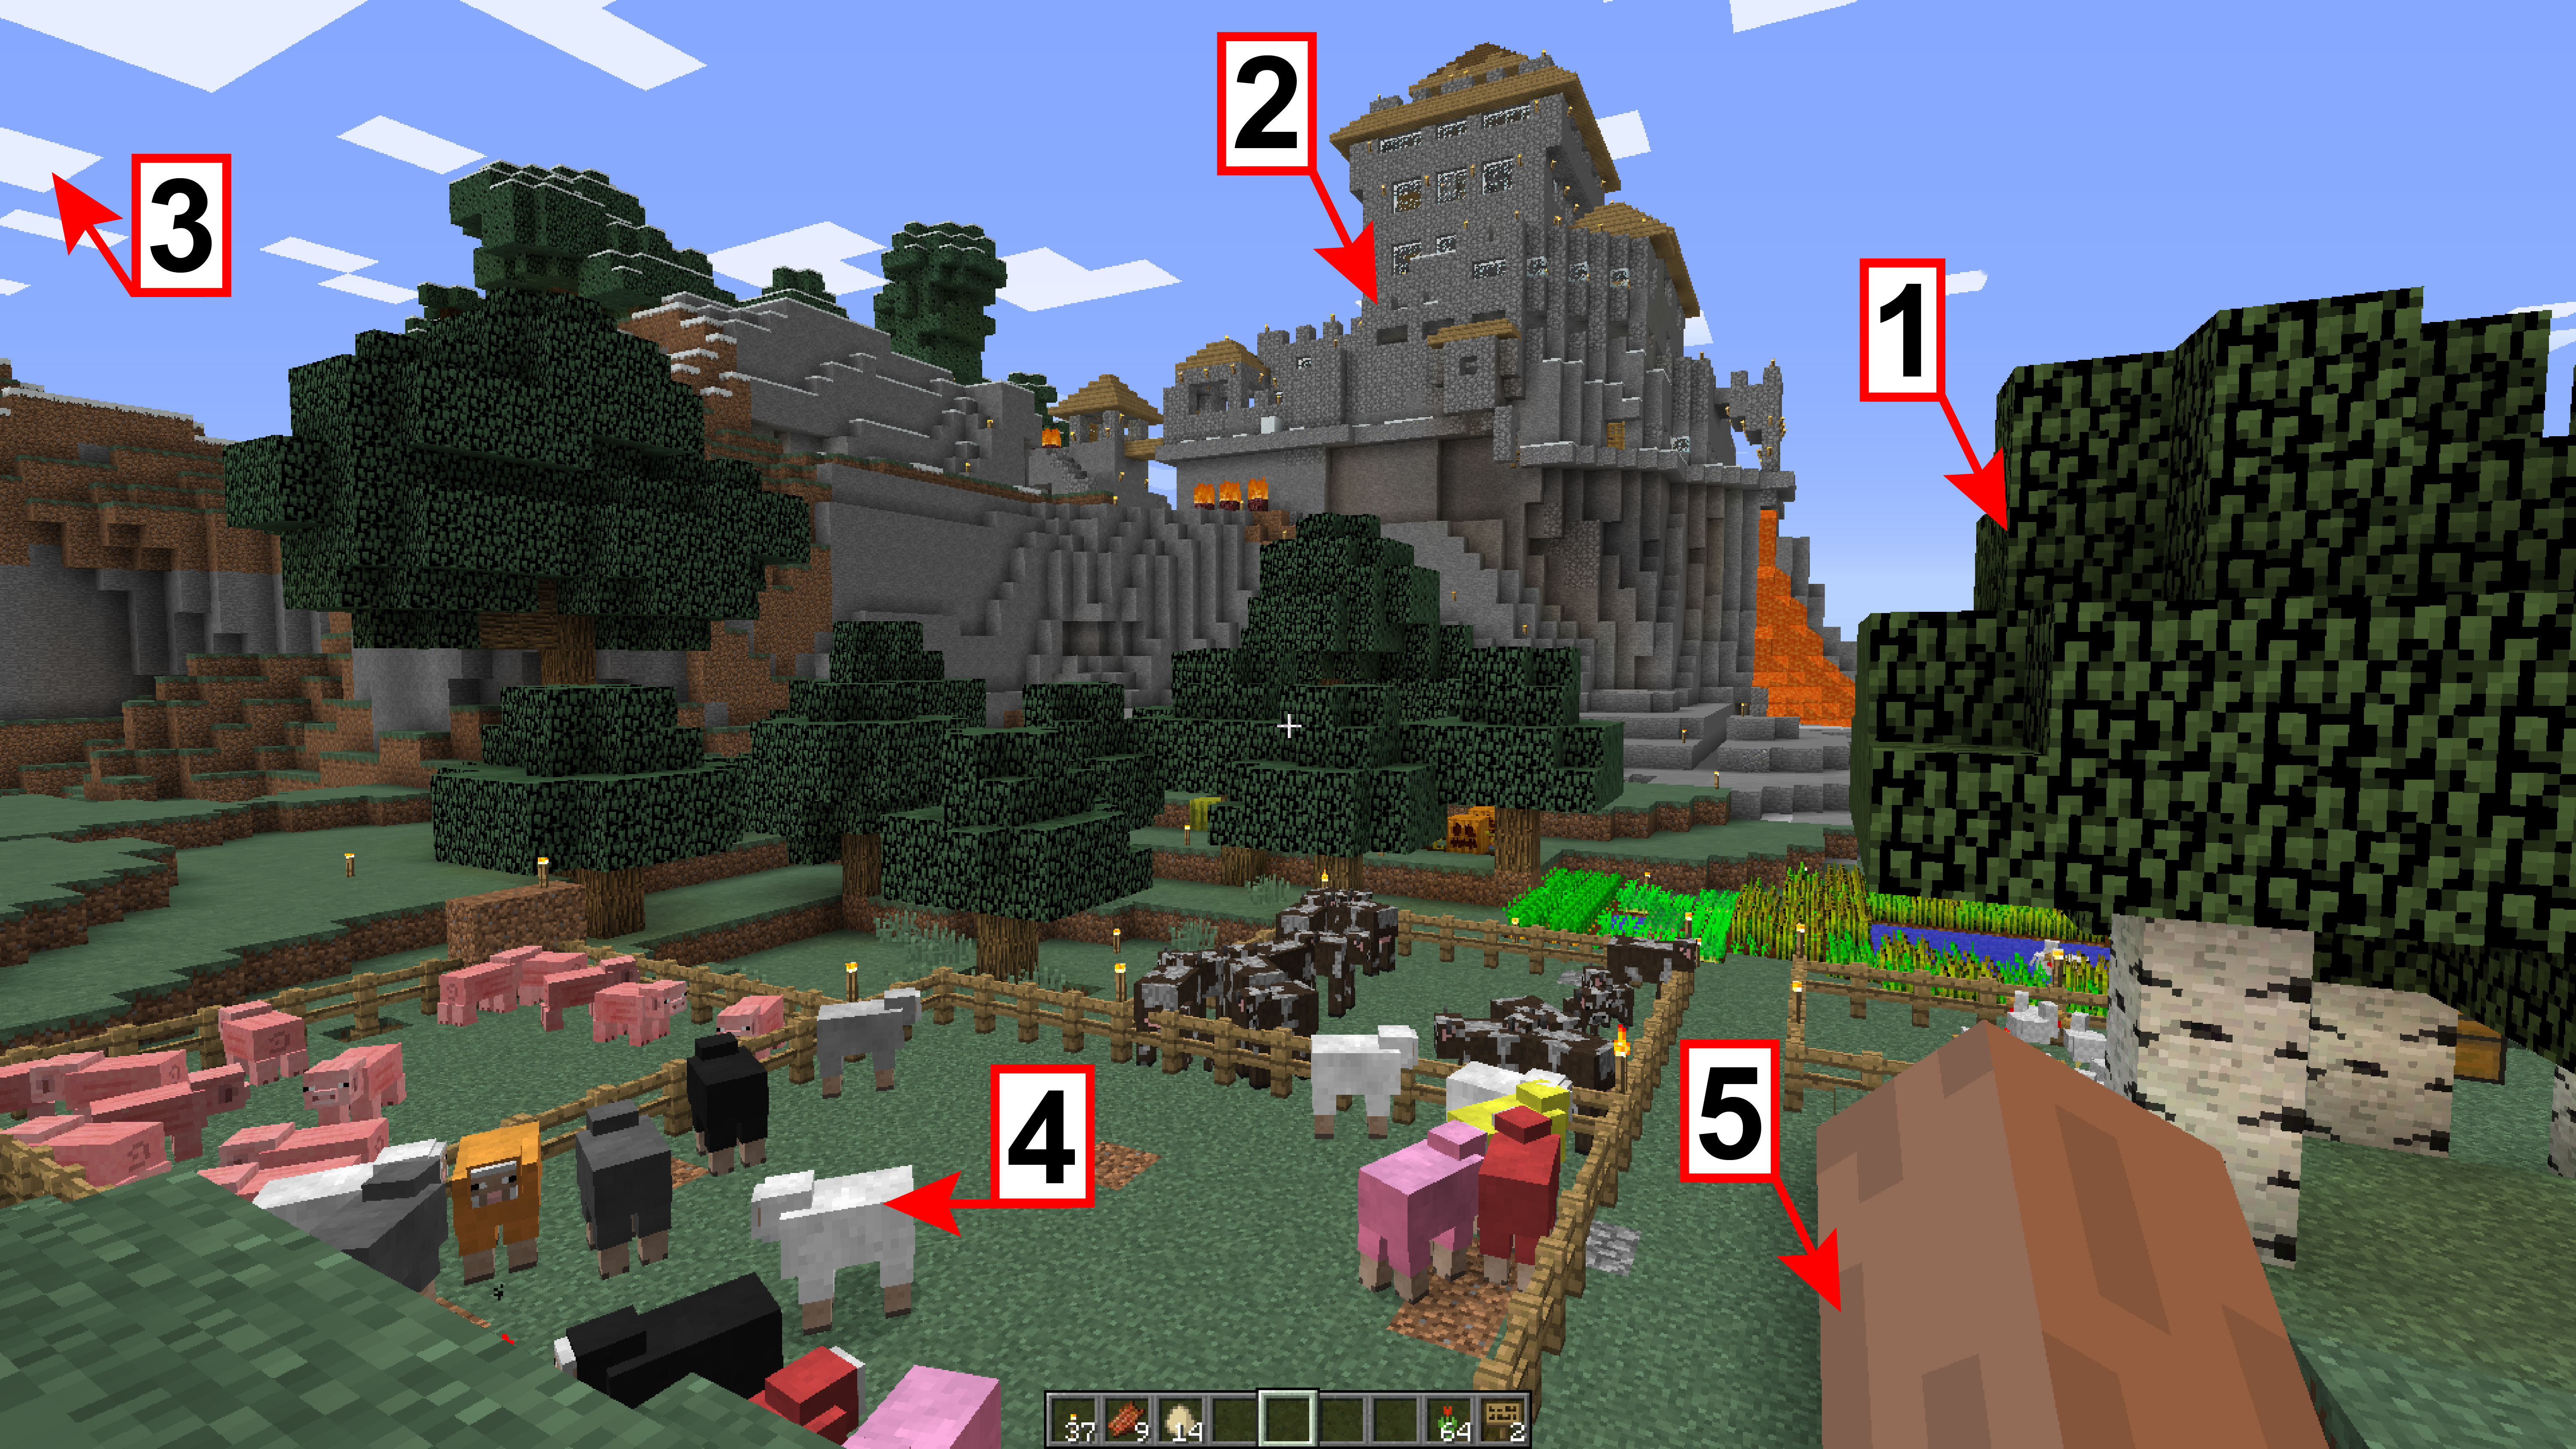
\includegraphics[ width=140mm]{../img/intro/mc}

\caption{Hra Minecraft -- hrad na skále}
\label{fig:intro_mc}

\end{figure}

\FloatBarrier

Ve hře \MC{} může hráč bloky umisťovat do herního světa. Bloky získává těžbou (například kutáním krumpáčem do kamenného bloku), nebo je může vyrobit tzv.~\textit{craftingem}. \textit{Crafting} probíhá skrze uživatelské rozhraní, kdy hráč z~nějaké kombinace herních bloků či obecně elementů vytváří nové bloky či elementy. \MC{} používá takový systém \textit{craftingu}, kdy hráč musí umístit bloky do konkrétního tvaru, aby získal nějaký nový objekt. 

Na obrázku \ref{fig:intro_crafting} můžeme vidět dvě varianty tvorby krumpáče. V jednom případě je hráčovým cílem vytvořit \textit{dřevěný krumpáč} (na obrázku vlevo), v~druhém případě pak \textit{kamenný krumpáč} (vpravo). Z toho důvodu v~prvním případě do vstupního tvaru umístí do horní části 3 bloky dřevěných prken, v~druhém případě použije 3 bloky kamení. Tímto způsobem je možné vytvářet nejen nástroje, ale i~zbraně, nové bloky a~dokonce i~jídlo, které pak hráč ve hře konzumuje.

\begin{figure}[!ht]\centering
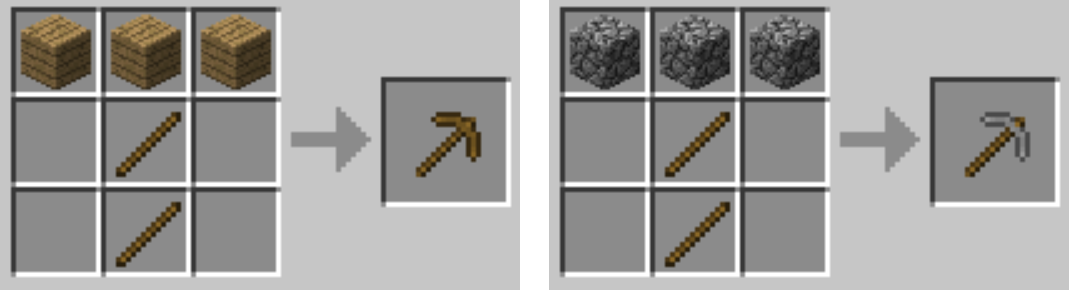
\includegraphics[ width=140mm]{../img/intro/crafting}

\caption{Hra Minecraft -- Crafting}
\label{fig:intro_crafting}

\end{figure}

\FloatBarrier

Stavění pak ve hře probíhá tak, že si hráč zvolí blok nebo objekt, který chce umístit do světa. Tento objekt musí mít ve svém inventáři. Namíří kurzor na už existující blok ve světě a~klikne levým tlačítkem myši. Ke straně bloku, na který hráč mířil, se pak připojí vybraný blok. Postavený blok se odebere z~inventáře a~dále nevyžaduje žádnou další akci (na rozdíl od jiných her, což si ukážeme v~následující sekci).


Mezi dalšími hrami bychom mohli zmínit například hru \TE{}. Ta je o~něco mladší než \MC{}, ale je častým zdrojem diskusí, zda je lepší než \MC{}, nebo ne. Pravdou je, že obě hry mají svůj svět kompletně složený z~kostek (\TE{} je však 2D hra), ale každá si klade trochu jiné cíle. \TE{} je více orientovaná na příběh, obsahuje více \NPC{} i~\textit{bossů}\footnote{\textit{Boss} je v~herní terminologii významný nepřítel, obvykle je silnější než ostatní protivníci a~velmi často bývá v~závěrečných částech hry. Duel s~\textit{bossem} pak obvykle od hráče vyžaduje zjištění jeho silných a~slabých stránek a~schémat jeho útoků~\citep{intro_boss}.}. \MC{} je pak orientován spíše na stavění (porovnání \textit{Minecraft vs Terraria (facts)}~\citep{mc_te_comparsion} na Minecraftovém fóru), ačkoliv od \textit{Combat update}, tedy verze 1.9, jsou možnosti boje oproti dřívějším verzím větší (stránka s~popisem aktualizace hry~\citep{mc_combat}). 


\subsection{Hry s~prvky realismu}

Mezi hry s~prvky realismu bychom mohli zařadit třeba hry \SE{} či \ME{}, využívající kombinaci herních bloků s~\textit{voxelovou} reprezentací světa (voxely si můžeme představit jako bloky stejné velikosti). Obě hry jsou implementovány v~proprietárním enginu společnosti Keen Software House nazvaném \textit{VRAGE}\texttrademark{}. Z voxelové reprezentace terénu je pak v~enginu za běhu hry procedurálně generovaná polygonální reprezentace terénu, kterou pak grafická karta standardním způsobem vykreslí na obrazovce (oficiální popis vlastností enginu~\citep{vrage}). Obdobným způsobem jako terén se pak ve hře \SE{} chovají různá vesmírná tělesa či asteroidy. Během procedurálního vytváření asteroidu je na třídimenzionální strukturu voxelů aplikován šum a~tím je možné ve hře vygenerovat prakticky neomezené množství různých asteroidů vycházejících z~jedné voxelové struktury. \uv{\textit{The “procedural asteroids” feature adds a~practically infinite number of asteroids to the game world}}~\citep{rosa_blog}. Tímto způsobem pak hry dosahují vyššího stupně realismu -- nespoléhají se pouze na předpřipravené 3D modely, ale generují vizuální reprezentaci herních objektů za běhu hry. Z toho vyplývá, že každý hráč může stejnou hru prožít jinak. 

Podívejme se na obrázek \ref{fig:intro_se} ze hry \SE{}. Na něm můžeme vidět převážně kamenný asteroid a~na něm je postavená vesmírná základna (1). K základně je přistavena větší vesmírná loď (2), hráč pak k~základně letí v~další, malé lodi (3). Můžeme si všimnout, že povrch asteroidu (4) není pravidelný a~obsahuje spoustu nerovností (na rozdíl od tvarů základny a~lodí). To je způsobeno právě algoritmickou aproximací voxelové reprezentace asteroidu. 

\begin{figure}[!ht]\centering
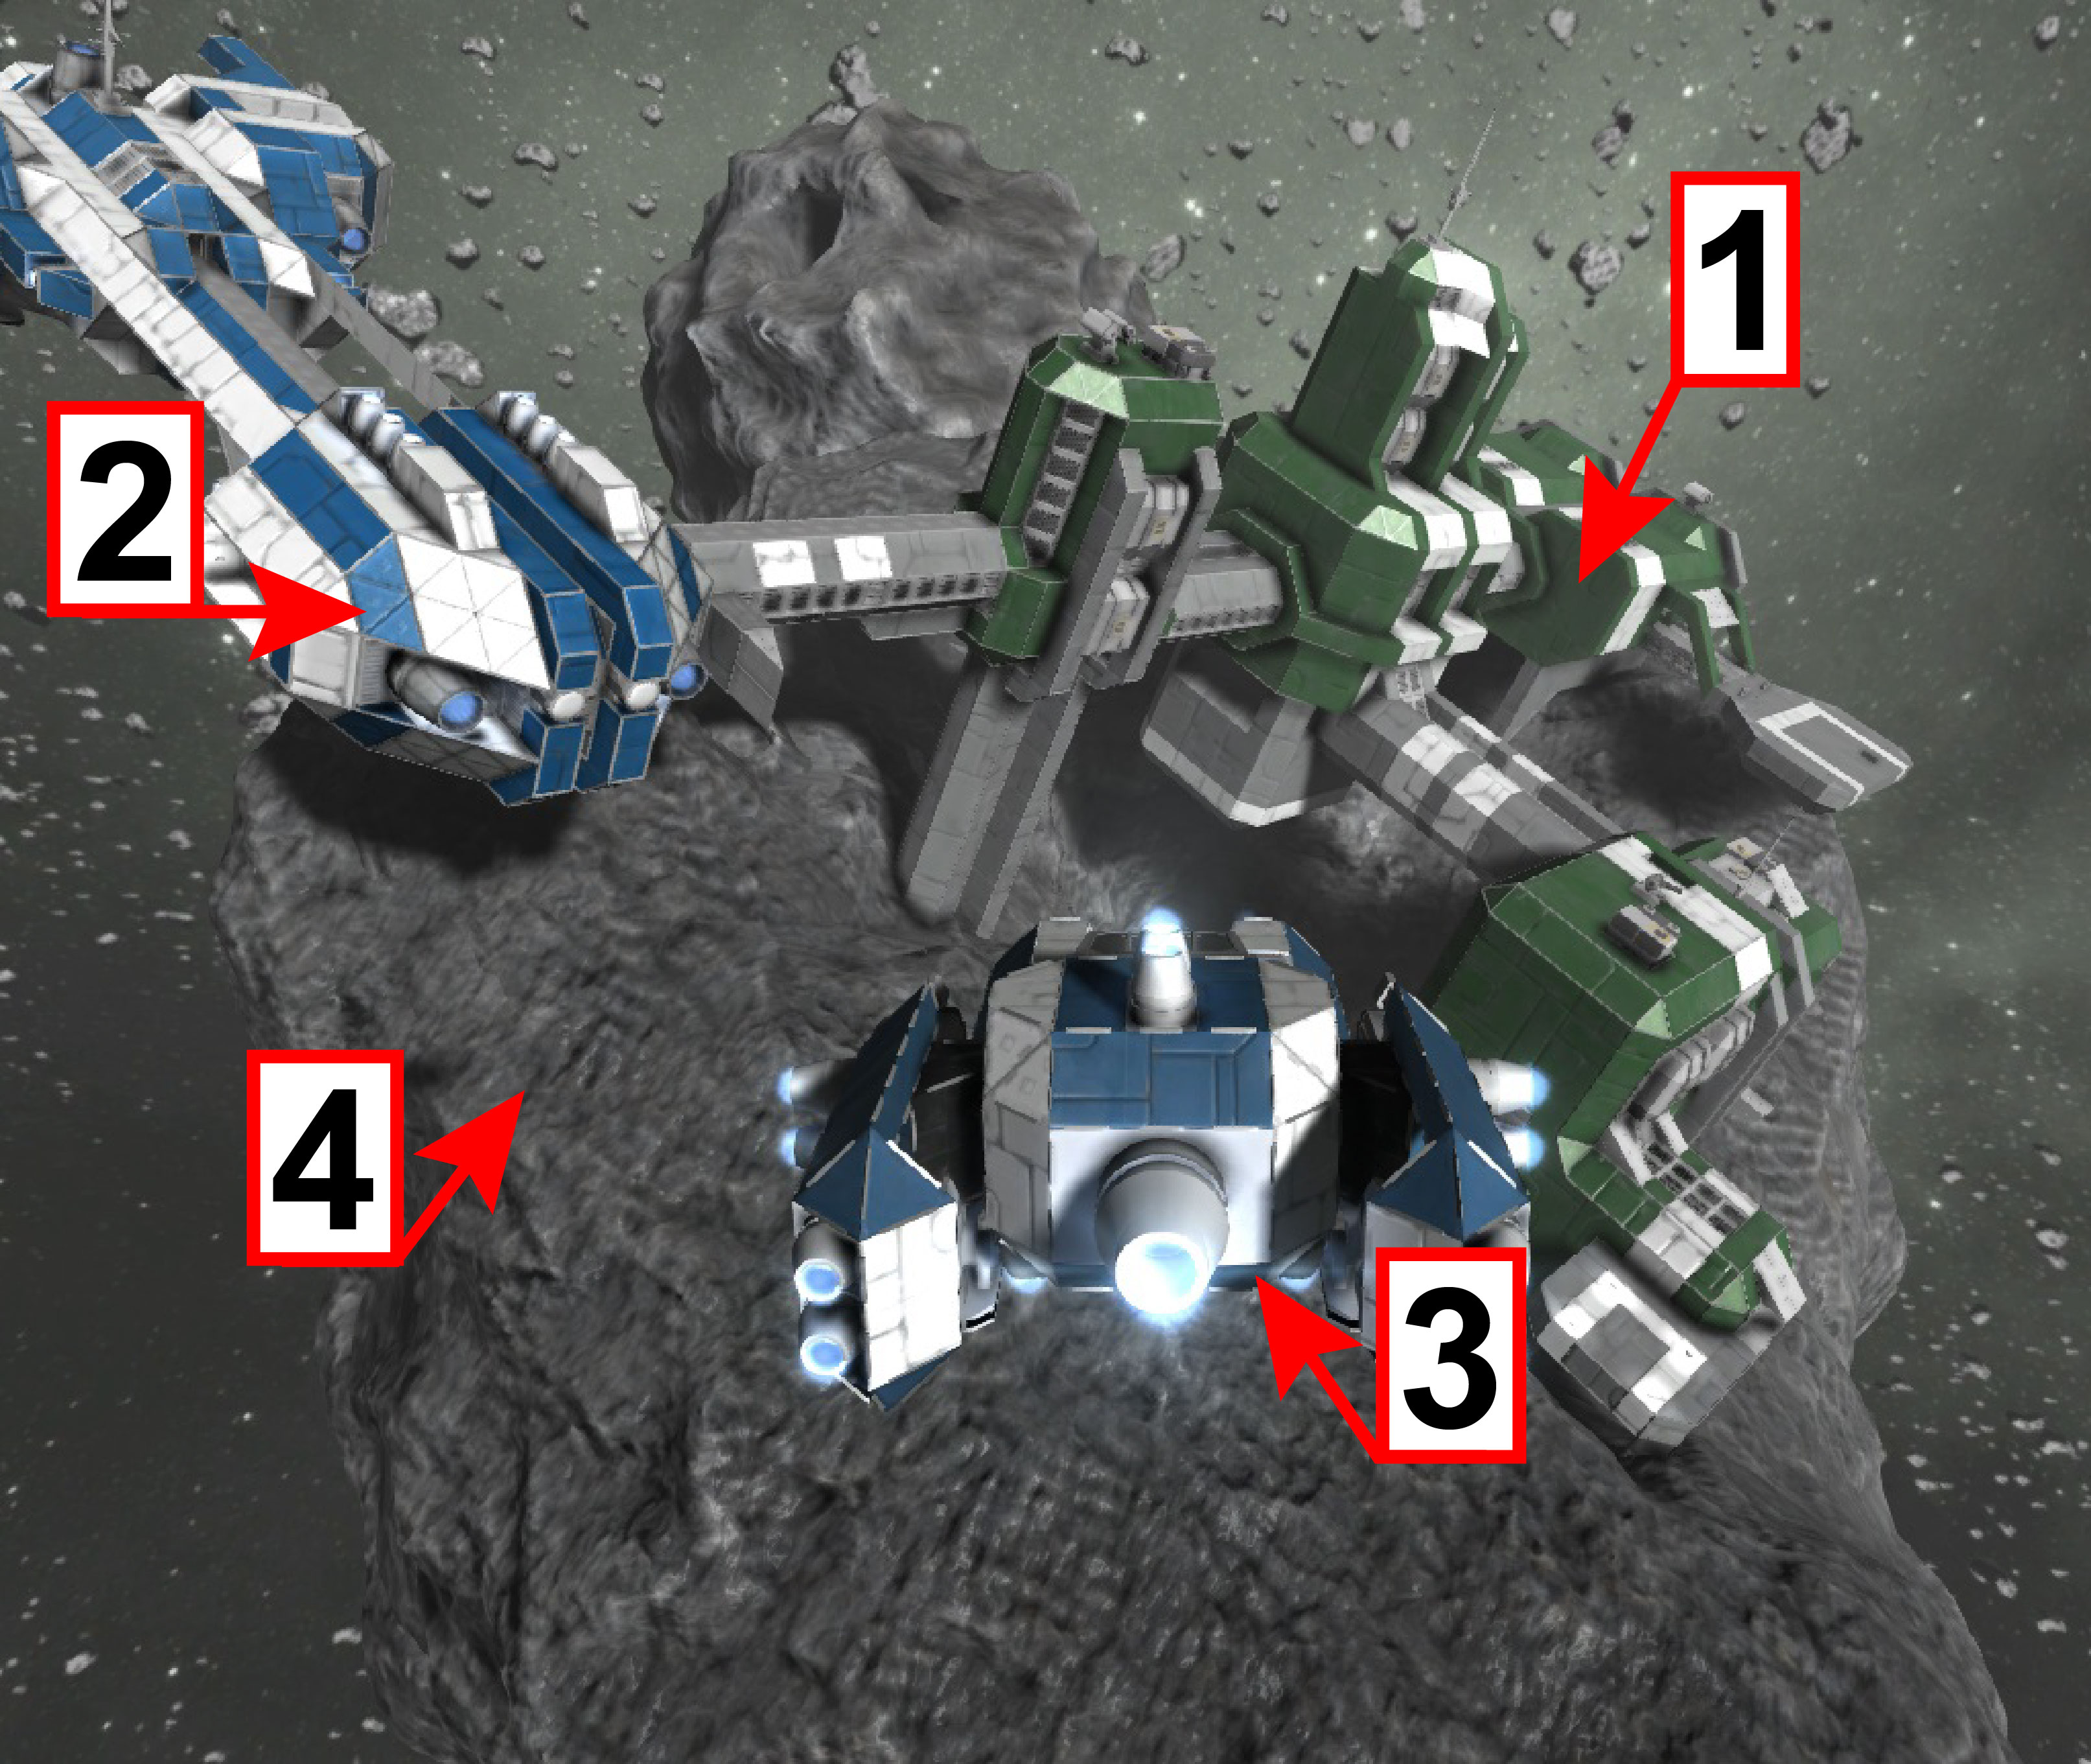
\includegraphics[ width=140mm]{../img/intro/se}

\caption{Hra Space Engineers -- základna. Zdroj: Gamespot.com~\citep{se_intro_img} }
\label{fig:intro_se}

\end{figure}

\FloatBarrier

Samotná základna i~vesmírná plavidla (detailní pohled na jiné plavidlo je na obrázku \ref{fig:intro_se_ship}) jsou tvořeny bloky. Vizuální reprezentace bloku může být i~jiného tvaru než jen krychle -- to je možné vidět na obrázku \ref{fig:intro_se_blocks}. Na stejném obrázku můžeme vidět barevně zvýrazněné hranice bloků. Jak základny, tak vesmírné lodě (které jsou navíc oproti základnám pohyblivé) využívají tento systém bloků. 

\begin{figure}[!ht]\centering
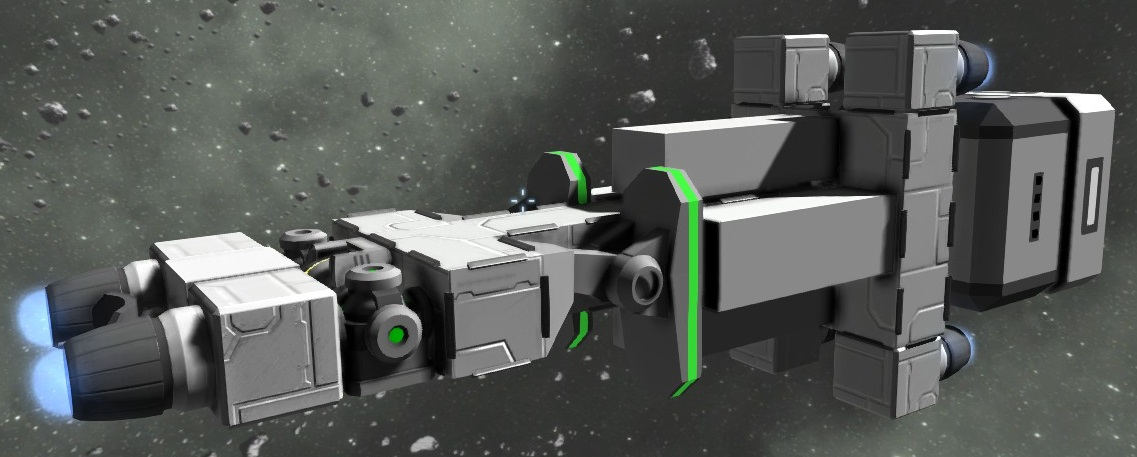
\includegraphics[ width=140mm]{../img/intro/se_ship}

\caption{Hra Space Engineers -- dron. Zdroj: space-engineer.net~\citep{se_drone_source}}
\label{fig:intro_se_ship}

\end{figure}

\begin{figure}[!ht]\centering
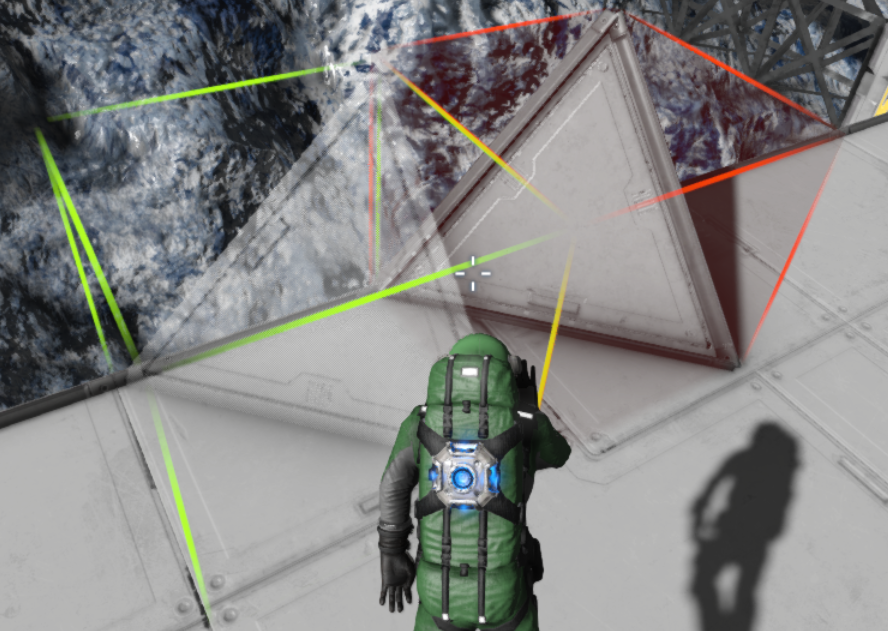
\includegraphics[ width=140mm]{../img/intro/se_blocks}

\caption{Hra Space Engineers -- bloky }
\label{fig:intro_se_blocks}

\end{figure}

\FloatBarrier


\SE{} umožňuje stavět pohyblivé stroje, které si hráč postaví z~herních bloků, jež se pak dohromady chovají jako jedna entita. Stále je na ně však aplikována fyzika, takže je možné plavidlo poškodit, nebo dokonce zničit. Obdobně lze ve hře \SE{} stavět různá mechanická obléhací zařízení, například pojízdné katapulty.

\textit{Crafting} v~podobě, ve které je použit ve hře \MC{}, se ve hře \SE{} neobjevuje, ale můžeme zde nalézt obdobný systém. Hráč musí těžit rudy, které pak dává do specializovaného stroje (bloku) na zpracování. V ovládacím rozhraní tohoto bloku si pak vybere, kterou součástku chce vytvořit. Tyto součástky jsou pak použity ke stavbě dalších bloků (zde je zásadní rozdíl se hrou \MC{}).

Stavění je ve hře \SE{} vyřešeno tak, že si hráč vybere z~nabídky všech dostupných bloků nějaký blok, který chce postavit. Tento stavěný blok můžeme chápat spíše jako návod, jak jej postavit, než jako fyzické umisťování bloku do herního světa (případ \MC{u}). Po umístění vybraného bloku do světa hráč uvidí pouze základní konstrukci vycházející z~tvaru bloku. Za použití specializovaného nástroje a~součástek ze svého inventáře pak po nějakou dobu \uv{staví} daný blok, přičemž v~průběhu tohoto stavění se spotřebovávají potřebné součástky z~hráčova inventáře a~zároveň se po nějakých krocích mění vizuální podoba stavěného bloku. Můžeme tedy říct, že \textit{crafting} se ve hře \SE{} neobjevuje v~podobě tvorby specifických tvarů v~uživatelském rozhraní a~následném získání předmětu, nýbrž v~podobě získávání prostředků pro tvorbu součástek, které jsou vyžadovány pro další stavbu.

Hra \ME{} implementuje systém stavění na pomezí her \MC{} a~\SE{}. Hráč nemá na začátku hry k~dispozici všechny bloky, ale může si postavit blok \textit{Výzkumného stolu}, ve kterém pak za nějakou cenu může znalost konstrukce nového bloku vyzkoumat. Z výzkumu vzejde svitek, který si hráč může přečíst a~tím se naučí stavět nový blok. Zajímavou vlastností hry je, že na multiplayerovém serveru je možné tyto svitky předávat dalším hráčům a~ti se pak mohou stavbu nového bloku naučit také, aniž by museli sami zkoumat stavbu daných bloků. Stavba pak dále funguje obdobným způsobem jako u~\SE{} s~tím rozdílem, že místo technických součástek se používají různé kamenné, dřevěné a~jiné další herní objekty. 




\subsection{Hry s~maximálním důrazem na simulaci reality}

Mezi hry s~maximálním důrazem na simulaci reality bychom mohli zařadit například vesmírný simulátor \TM{}. Tato hra si klade za cíl se maximálně přiblížit zážitku, který by mohli astronauti zažít při cestách na Měsíc a~na Mars. Bloky se zde objevují v~podobě standardizovaných částí budov, ale třeba vozidla jsou kompletně vymodelována a~hráč je nemůže stavět ani nijak modifikovat. Představu o~hře si můžeme udělat z~obrázku \ref{fig:intro_tom}.

\begin{figure}[!ht]\centering
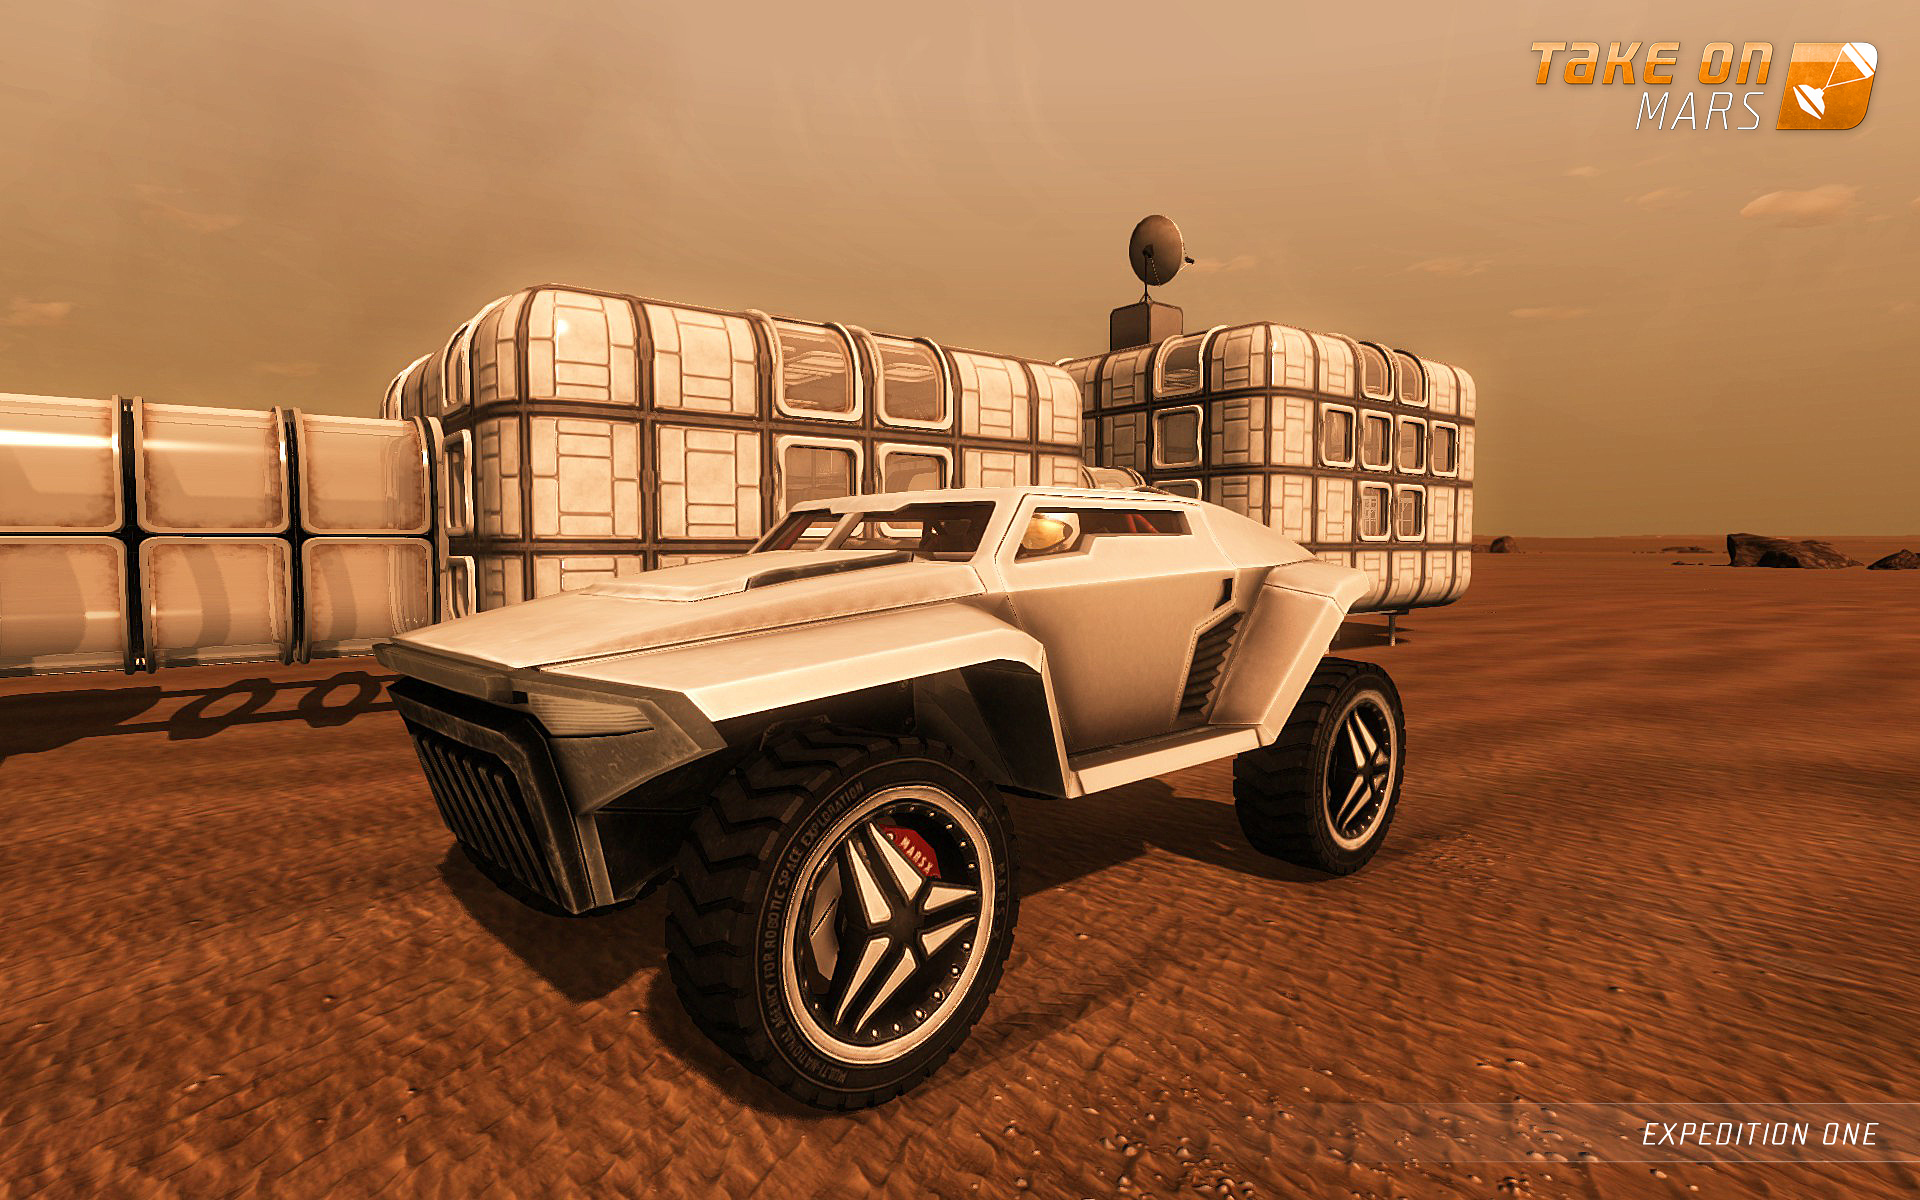
\includegraphics[ width=140mm]{../img/intro/tom}

\caption{Hra Take On Mars -- vozítko před budovou. Zdroj: Hry.cz~\citep{intro_tom_source}}
\label{fig:intro_tom}

\end{figure}

\FloatBarrier

Stavění ve hře \TM{} probíhá tak, že hráč přidává bloky k~už postaveným blokům na konkrétní, vývojáři definované přípojné body. To má výhodu v~tom, že hra snadno pozná, že je stavba někde \uv{děravá}. Pokud je někde ve struktuře stavby netěsnost, pak například neprobíhá okysličení a~natlakování vnitřních prostor takovéto nedokončené stavby. 

Hra dále nabízí možnost vytváření nových bloků a~objektů dvěma způsoby. V rámci \textit{kreativní} hry (tedy hry bez omezení) má hráč k~dispozici speciální \textit{3D tiskárnu}, která umí \uv{vytisknout} libovolný herní objekt (a to dokonce bez jakýchkoliv nákladů). Později do hry přibyl druhý způsob, použitelný v~\textit{běžné} hře -- \textit{konstruktor objektů}. Ten je složen z~několika bloků a~je možné díky němu \uv{vytisknout} třeba celé vozidlo. Velikost výsledných objektů je omezena velikostí konstruktoru, tudíž není možné vytvářet objekty větší, než je velikost konstruktoru (bráno vnitřními rozměry).

\TM{} taktéž používá systém těžby a~zpracování nerostů a~minerálů, které slouží jako zdroj surovin pro konstruktor objektů. Suroviny jsou plněny do speciálních kontejnerů, ze kterých mohou být opětovně spotřebovávány na stavbu.

\subsection{Možné další inspirace }
Námi zmíněné hry rozhodně nejsou všechny dostupné hry. Stále vznikají nové hry a~ty stávající se postupně upravují a~vylepšují. Navíc mnohé z~nich jsou v~různých fázích vývoje (Alfa či Beta verze), a~tak se situace velice rychle mění. Rádi bychom však zmínili ještě některé další hry, které nás sice zaujaly, ale kromě různých variant prostředí obvykle nepřináší žádnou novou a~zásadní funkcionalitu.

% https://www.youtube.com/watch?v=d2ySkvn6wyw
Hra \NI{} patří do žánru \textit{MMORPG} (\textit{massively multiplayer online role-playing game} -- onlinová hra na hrdiny s~velkým množstvím hráčů). Na této hře bychom rádi zmínili koncept stavění, který probíhá poměrně netradičně. Hráč se přepne do stavitelského módu a~celou stavbu si naplánuje. V tomto plánovači vidí výsledek rovnou tak, jak bude budova po dokončení vypadat. Bloky se během stavění přichytávají do mřížky a~k~sobě. Po ukončení toho módu pak hráč vidí obrysy naplánovaných bloků. Pak je může začít konstruovat, přičemž v~nabídce (během konstrukce) má možnost si chybějící součásti vytvořit pomocí \textit{craftingu}. V tomto ohledu je to tedy podobné \SE{}. Plánovač se nám sice líbí, ale zastáváme názor, že je to pouze pomůcka, bez které je možné se obejít. Ostatně bloky lze kupříkladu ve \SE{} stavět i~na nedokončených blocích a~později, až je výsledná hrubá stavba hotová ke hráčově spokojenosti, je všechny dokončit specializovaným nástrojem.


%https://www.youtube.com/watch?v=Wpurqr3YaGQ 
Hra \PN{} funguje podobně jako \SE{} -- získávání surovin, jejich crafting na komponenty a~používání komponent na konstrukci objektů. Nově postavený (nedokončený) objekt ukazuje základní konstrukci a~komponenty nutné k~dokončení. Stejně jako u~\SE{} je zde možné vytvářet pohyblivá vozidla, měnit terén apod. Z pohledu stavění tedy nepřináší nic nového. Hra navíc kromě velice hezké grafiky řeší vlastnosti herní postavy -- pokud hráč nějakou činnost vykonává opakovaně, tak se v~ní zlepšuje a~naopak -- a~tím se výrazně odlišuje od jiných her.


% https://www.youtube.com/watch?v=TOmjjo5QoP8 
Hra \ARK{} je pak opět podobnou kombinací předchozích her a~liší se jiným prostředí. Taktéž využívá při stavění systém přípojných bodů.

Hra \NMS{} je opět podobná předchozím, stavění využívá systém přípojných bodů. Hra má hezky řešený systém multibloků, kdy je možné upravit některé části staveb. Takže například místo zdi je možné vytvořit okno. Svojí funkcionalitou je tedy podobná hře \SE{}.

Abychom výše uvedeným hrám v~této kapitole nekřivdili, musíme zmínit fakt, že hry nejsou úplně stejné. Mnohé využívají třeba systém procedurálně generovaných planet a~každá hra se snaží v~něčem odlišit. Nicméně my se tímto aspektem (procedurálním generováním) zabývat nebudeme a~tedy pro účely naší práce můžeme výše zmíněné hry považovat za podobné.

\section{Čemu se budeme věnovat}
V této práci bychom rádi navrhli a~posléze implementovali nové přístupy a~herní mechaniky, které by měly usnadnit stavění ve stavitelských hrách. Rádi bychom zachovali koncept použití herních bloků, který shledáváme jednoduchý na pochopení i~použití. Zaměříme se na rozšíření možnosti práce s~bloky tak, abychom hráči nabídli, pokud možno, ještě lepší herní zážitek ze stavění vlastních výtvorů. V této práci se nebudeme nijak důkladně věnovat vizuální reprezentaci prostředí, protože ta pro nás v~tuto chvíli není podstatná.

Změna v~přístupu k~herním blokům bude vyžadovat i~úpravy herního mechanismu s~tím souvisejícího -- hráčova inventáře. Všechny výše zmíněné hry nějakým způsobem nabízí hráči výběr bloků, které může do herního světa umístit. Naše změna by bohužel znamenala, že by se takový inventář postavitelných bloků velmi rychle stal nepřehledným a~proto musíme systém nabídky postavitelných bloků upravit pro naše potřeby.


\section{Herní bloky}
Obvykle je ve hře definován jeden základní rozměr bloku, který je neměnný\footnote{\SE{} definuje více velikostí -- ty však nelze vzájemně kombinovat}. To však může být problémem, pokud se hráč rozhodne postavit v~herním světě nějakou větší a~komplexnější strukturu podle reálné či fiktivní předlohy. Pro příklad uveďme některé výtvory ze hry \MC{} -- město Královo přístaviště z~knih Píseň ledu a~ohně od George R. R. Martina, nebo hlavní město Gondoru Minas Tirith z~knih Pána prstenů od J. R. R. Tolkiena. Autoři těchto výtvorů museli volit takové měřítko, aby byly výtvory dostatečně detailní, ale zároveň aby bylo možné výtvor postavit v~nějakém rozumném čase. Obecně můžeme říct, že čím větších detailů chtějí autoři ve hře \MC{} dosáhnout, tím větší musí celý výtvor být. To pak ale znamená, že celá stavba trvá déle, nebo je zapotřebí více spolupracujících hráčů. 

Hra \SE{} a~jí podobné díky svému přístupu a~více bloků, které nejsou tvaru krychle, nabízí lepší možnosti staveb rozsáhlých objektů (představme si třeba Hvězdu smrti z~Hvězných válek), ale stále je potřeba volit nějakou rozumnou výslednou velikost. Možnosti detailů se sice zvyšují s~rostoucím počtem různých vizuálních variant bloků (což je třeba případ \SE{} nebo \NI{}), ale i~tak bychom chtěli navrhnout nový systém, ve kterém lze používat bloky různých velikostí.




\subsubsection{Náš návrh úpravy}
Chtěli bychom se v~této práci zabývat myšlenkou proměnlivé velikosti stavitelných bloků. Tím by hráči mohli rychleji stavět rozsáhlejší struktury a~přitom se věnovat i~drobným či estetickým detailům. Tento návrh však s~sebou nese několik problémů, které se v~této práci budeme snažit vyřešit.

Ačkoliv se nám idea postupné stavby bloku ze součástek velice líbí, od naší hry tuto funkcionalitu nebudeme požadovat. Znamenalo by to pro nás, že bychom museli řešit vizuální podobu rozpracovaných bloků, navíc v~kombinaci s~různými rozměry. Pak bychom nejspíše museli generovat tyto objekty procedurálně, přičemž realizace této vlastnosti by nám zabrala velké množství času. Implementaci této funkcionality tedy vidíme (v současné době) jako zbytečnou, protože nevíme, zda vůbec bude myšlenka proměnlivé velikosti bloků přijata hráči.


\section{Inventář}
Dalším společným prvkem stavitelských her je inventář bloků, které může hráč umístit do herního světa. Hráč vidí přes celé herní okno \HUD{} (Head-Up Display~\citep{hud_terminology}), ve kterém má zobrazenou kromě jiného nabídku bloků, které má na rychlé volbě, může je snadno zvolit a~daný blok umístit do herního světa. Navíc hry mohou definovat i~inventární skupiny bloků (\SE{}, \ME{}), mezi kterými hráč může přepínat a~tím rychle kompletně změnit sadu rychlé nabídky. Vidíme však limitaci v~tom, že hráč musí ručně spravovat tyto seznamy a~jednotlivé bloky (či nástroje) ručně umisťovat do příslušných pozic, například pomocí systému Drag and Drop (tedy přetáhnutí bloku myší z~nabídky inventáře do rychlé volby stavitelných bloků).


\subsubsection{Náš návrh úpravy}
Rádi bychom navrhli jiný způsob správy těchto inventárních skupin tak, aby hráč jednou definoval, jaké prvky chce mít v~příslušných skupinách. Při vytvoření nového bloku či vytvoření jiné velikosti bloku by pak nemusel ručně přiřazovat nový blok do skupiny, ale tento blok by měl být automaticky zařazen a~nabídnut hráči. 


\section{Cíle práce}
\label{sec:cile}
Tato práce bude mít dvě fáze. V první fázi provedeme analýzu současného stavu a~možných řešení, ze které nám vzejdou podrobnější cíle práce. Druhá fáze práce pak bude implementace hry jako takové. Naše cíle tedy jsou:

\begin{enumerate}

 \item Analytická část
\begin{itemize}
	\item Navrhnout způsob řešení proměnlivé velikosti bloků
	\item Navrhnout automatizovanou správu inventáře
	\item Navrhnout celkovou koncepci hry vzhledem k~předchozím bodům
\end{itemize}

 \item Implementační část
\begin{itemize}
	\item Implementovat navržený způsob řešení proměnlivé velikosti bloků
	\item Implementovat automatizovanou správu inventáře
	\item Implementovat zbylé koncepty a~cíle hry, vzešlé z~\ref{chap:analyza}. kapitoly
	\item Kvůli očekávaným nárokům na pochopení nových konceptů do hry implementovat základní výukový tutoriál
	\item Získat a~zhodnotit zpětnou vazbu (dotazník) na výslednou hru
\end{itemize}

\end{enumerate}


